
%(BEGIN_QUESTION)
% Copyright 2010, Tony R. Kuphaldt, released under the Creative Commons Attribution License (v 1.0)
% This means you may do almost anything with this work of mine, so long as you give me proper credit

Suppose we have an Allen-Bradley MicroLogix 1000 controller connected to a pair of momentary-contact pushbutton switches and contactor controlling power to an electric motor as shown in this illustration:

$$\includegraphics[width=15.5cm]{i04530x01.eps}$$

This motor control system has a problem, though: the motor refuses to start when the ``Start'' pushbutton is pressed.  Examine the ``live'' display of the ladder logic program inside this Allen-Bradley PLC to determine what the problem is, assuming an operator is continuously pressing the ``Start'' pushbutton as you examine the program:

$$\includegraphics[width=15.5cm]{i04530x02.eps}$$

Identify at least two wiring faults that could account for all you see here.

\underbar{file i04530}
%(END_QUESTION)





%(BEGIN_ANSWER)


%(END_ANSWER)





%(BEGIN_NOTES)

Input {\tt I:0/2} is not activated as it should be, which means there is most likely an ``open'' wire fault between that input terminal on the PLC and the ``Stop'' switch, or perhaps the ``Stop'' switch itself is failed open.

\vskip 20pt \vbox{\hrule \hbox{\strut \vrule{} {\bf Virtual Troubleshooting} \vrule} \hrule}

This question is a good candidate for a ``Virtual Troubleshooting'' exercise.  Presenting the diagram to students, you first imagine in your own mind a particular fault in the system.  Then, you present one or more symptoms of that fault (something noticeable by an operator or other user of the system).  Students then propose various diagnostic tests to perform on this system to identify the nature and location of the fault, as though they were technicians trying to troubleshoot the problem.  Your job is to tell them what the result(s) would be for each of the proposed diagnostic tests, documenting those results where all the students can see.

During and after the exercise, it is good to ask students follow-up questions such as:

\begin{itemize}
\item{} What does the result of the last diagnostic test tell you about the fault?
\item{} Suppose the results of the last diagnostic test were different.  What then would that result tell you about the fault?
\item{} Is the last diagnostic test the best one we could do?
\item{} What would be the ideal order of tests, to diagnose the problem in as few steps as possible?
\end{itemize}










\vfil \eject

\noindent
{\bf Prep Quiz:}

Identify the stimulus condition of each switch in this PLC system, based on the color highlighting seen in the ladder-logic PLC program:

$$\includegraphics[width=15.5cm]{i04530x03.eps}$$

Pressure = {\it high} or {\it low}? \hskip 40pt Temperature = {\it high} or {\it low}? \hskip 40pt Level = {\it high} or {\it low}?









\vfil \eject

\noindent
{\bf Prep Quiz:}

Identify the stimulus condition of each switch in this PLC system, based on the color highlighting seen in the ladder-logic PLC program:

$$\includegraphics[width=15.5cm]{i04530x04.eps}$$

Pressure = {\it high} or {\it low}? \hskip 40pt Temperature = {\it high} or {\it low}? \hskip 40pt Level = {\it high} or {\it low}?









\vfil \eject

\noindent
{\bf Prep Quiz:}

Identify the stimulus condition of each switch in this PLC system, based on the color highlighting seen in the ladder-logic PLC program:

$$\includegraphics[width=15.5cm]{i04530x05.eps}$$

Pressure = {\it high} or {\it low}? \hskip 40pt Temperature = {\it high} or {\it low}? \hskip 40pt Level = {\it high} or {\it low}?



%INDEX% PLC, relating I/O status to virtual elements (troubleshooting)

%(END_NOTES)


